\section{并行计算与优化}

\subsection{GPU架构}

\paragraph{GPU简介}

\par GPU(Graphics Processing Unit)是一种高度并行结构,设计用于处理大规模的数据并行任务,
如图形渲染和科学计算。近年来也广泛应用于高性能计算和机器学习等领域。GPU由数百到数千个并行
处理核心组成,这些核心被组织在一个或多个流处理器(Streaming Multiprocessor,SM)中。
这些执行单元都是按照单指令多数据流方式运行的,即它们都执行相同的指令,但是对应于
不同的数据。因此,与CPU相比,GPU有着极高的并行处理能力,能够同时处理大量的并行任务。图\ref{fig:a100}和图\ref{fig:4090}展示了NVIDIA两款最新型号的GPU。

\begin{figure}[htb]
    \centering
    \begin{minipage}[t]{0.45\textwidth}
    \centering
    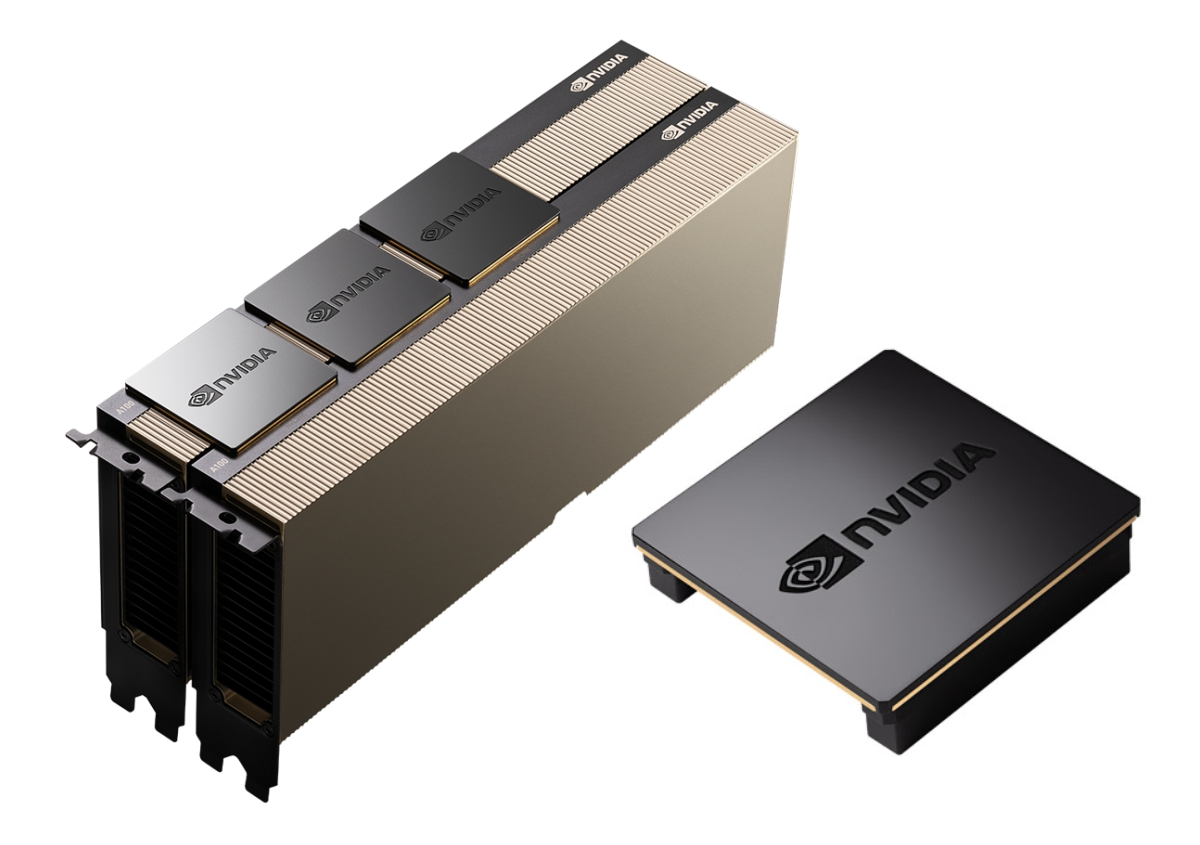
\includegraphics[height=4cm,keepaspectratio]{figures/a100.png}
    \caption{NVIDIA A100 Tensor Core GPU}
    \label{fig:a100}
    \end{minipage}
    % \hspace{1in}
    \begin{minipage}[t]{0.45\textwidth}
    \centering
    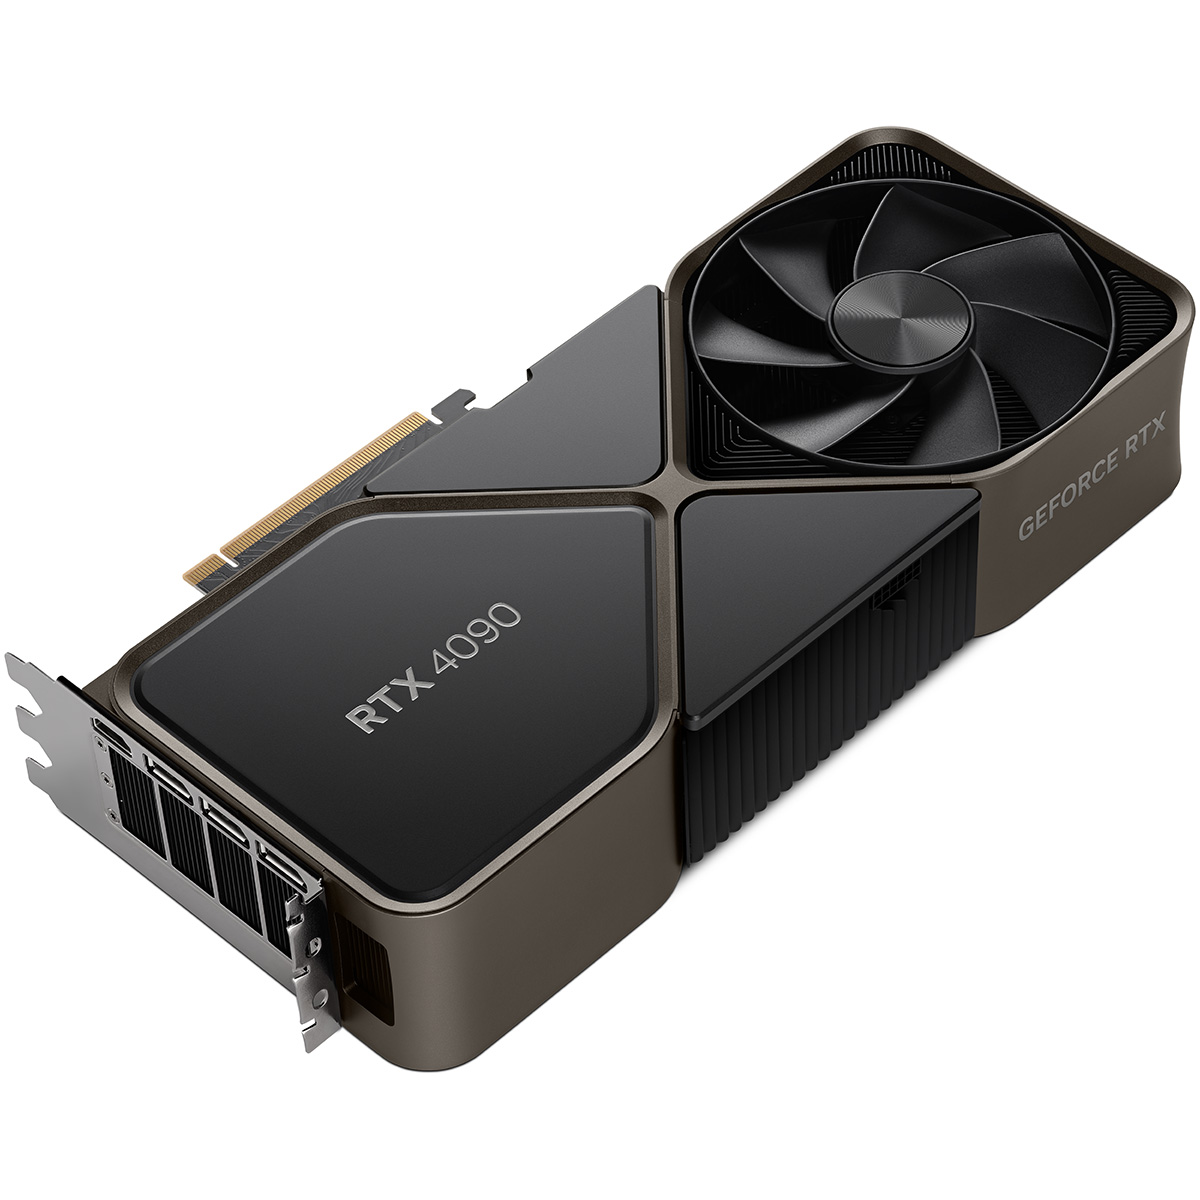
\includegraphics[height=4cm,keepaspectratio]{figures/4090.jpg}
    \caption{GeForce RTX 4090}
    \label{fig:4090}
    \end{minipage}
\end{figure}

\paragraph{GPU内存模型}

\par 如图\ref{fig:memory_hierarchy}\cite{nvidia_cuda}所示,GPU的内存模型是分层次的,包括全局内存(Global 
Memory)、共享内存(Shared Memory)、常量内存(Constant Memory)和纹理内存(Texture 
Memory)等。全局内存具有较大的存储容量,所有的线程都可以进行读写,但访问延迟较高。

\par GPU在运行时,首先从全局内存中读取数据,然后在各自的处理核心上执行一系列的指令,最后
将结果写回全局内存。共享内存提供给单个SM中的线程使用,具有较低的访问延迟,但容量较小。
常量内存和纹理内存主要用于读取操作,并且能通过缓存提高读取性能。另外,每个线程都拥有一些
私有的寄存器,用于存储临时的计算结果。当寄存器用完时,数据会溢出到本地内存。

\begin{figure}[htb]
    \centering
    \begin{minipage}[t]{0.55\textwidth}
    \centering
    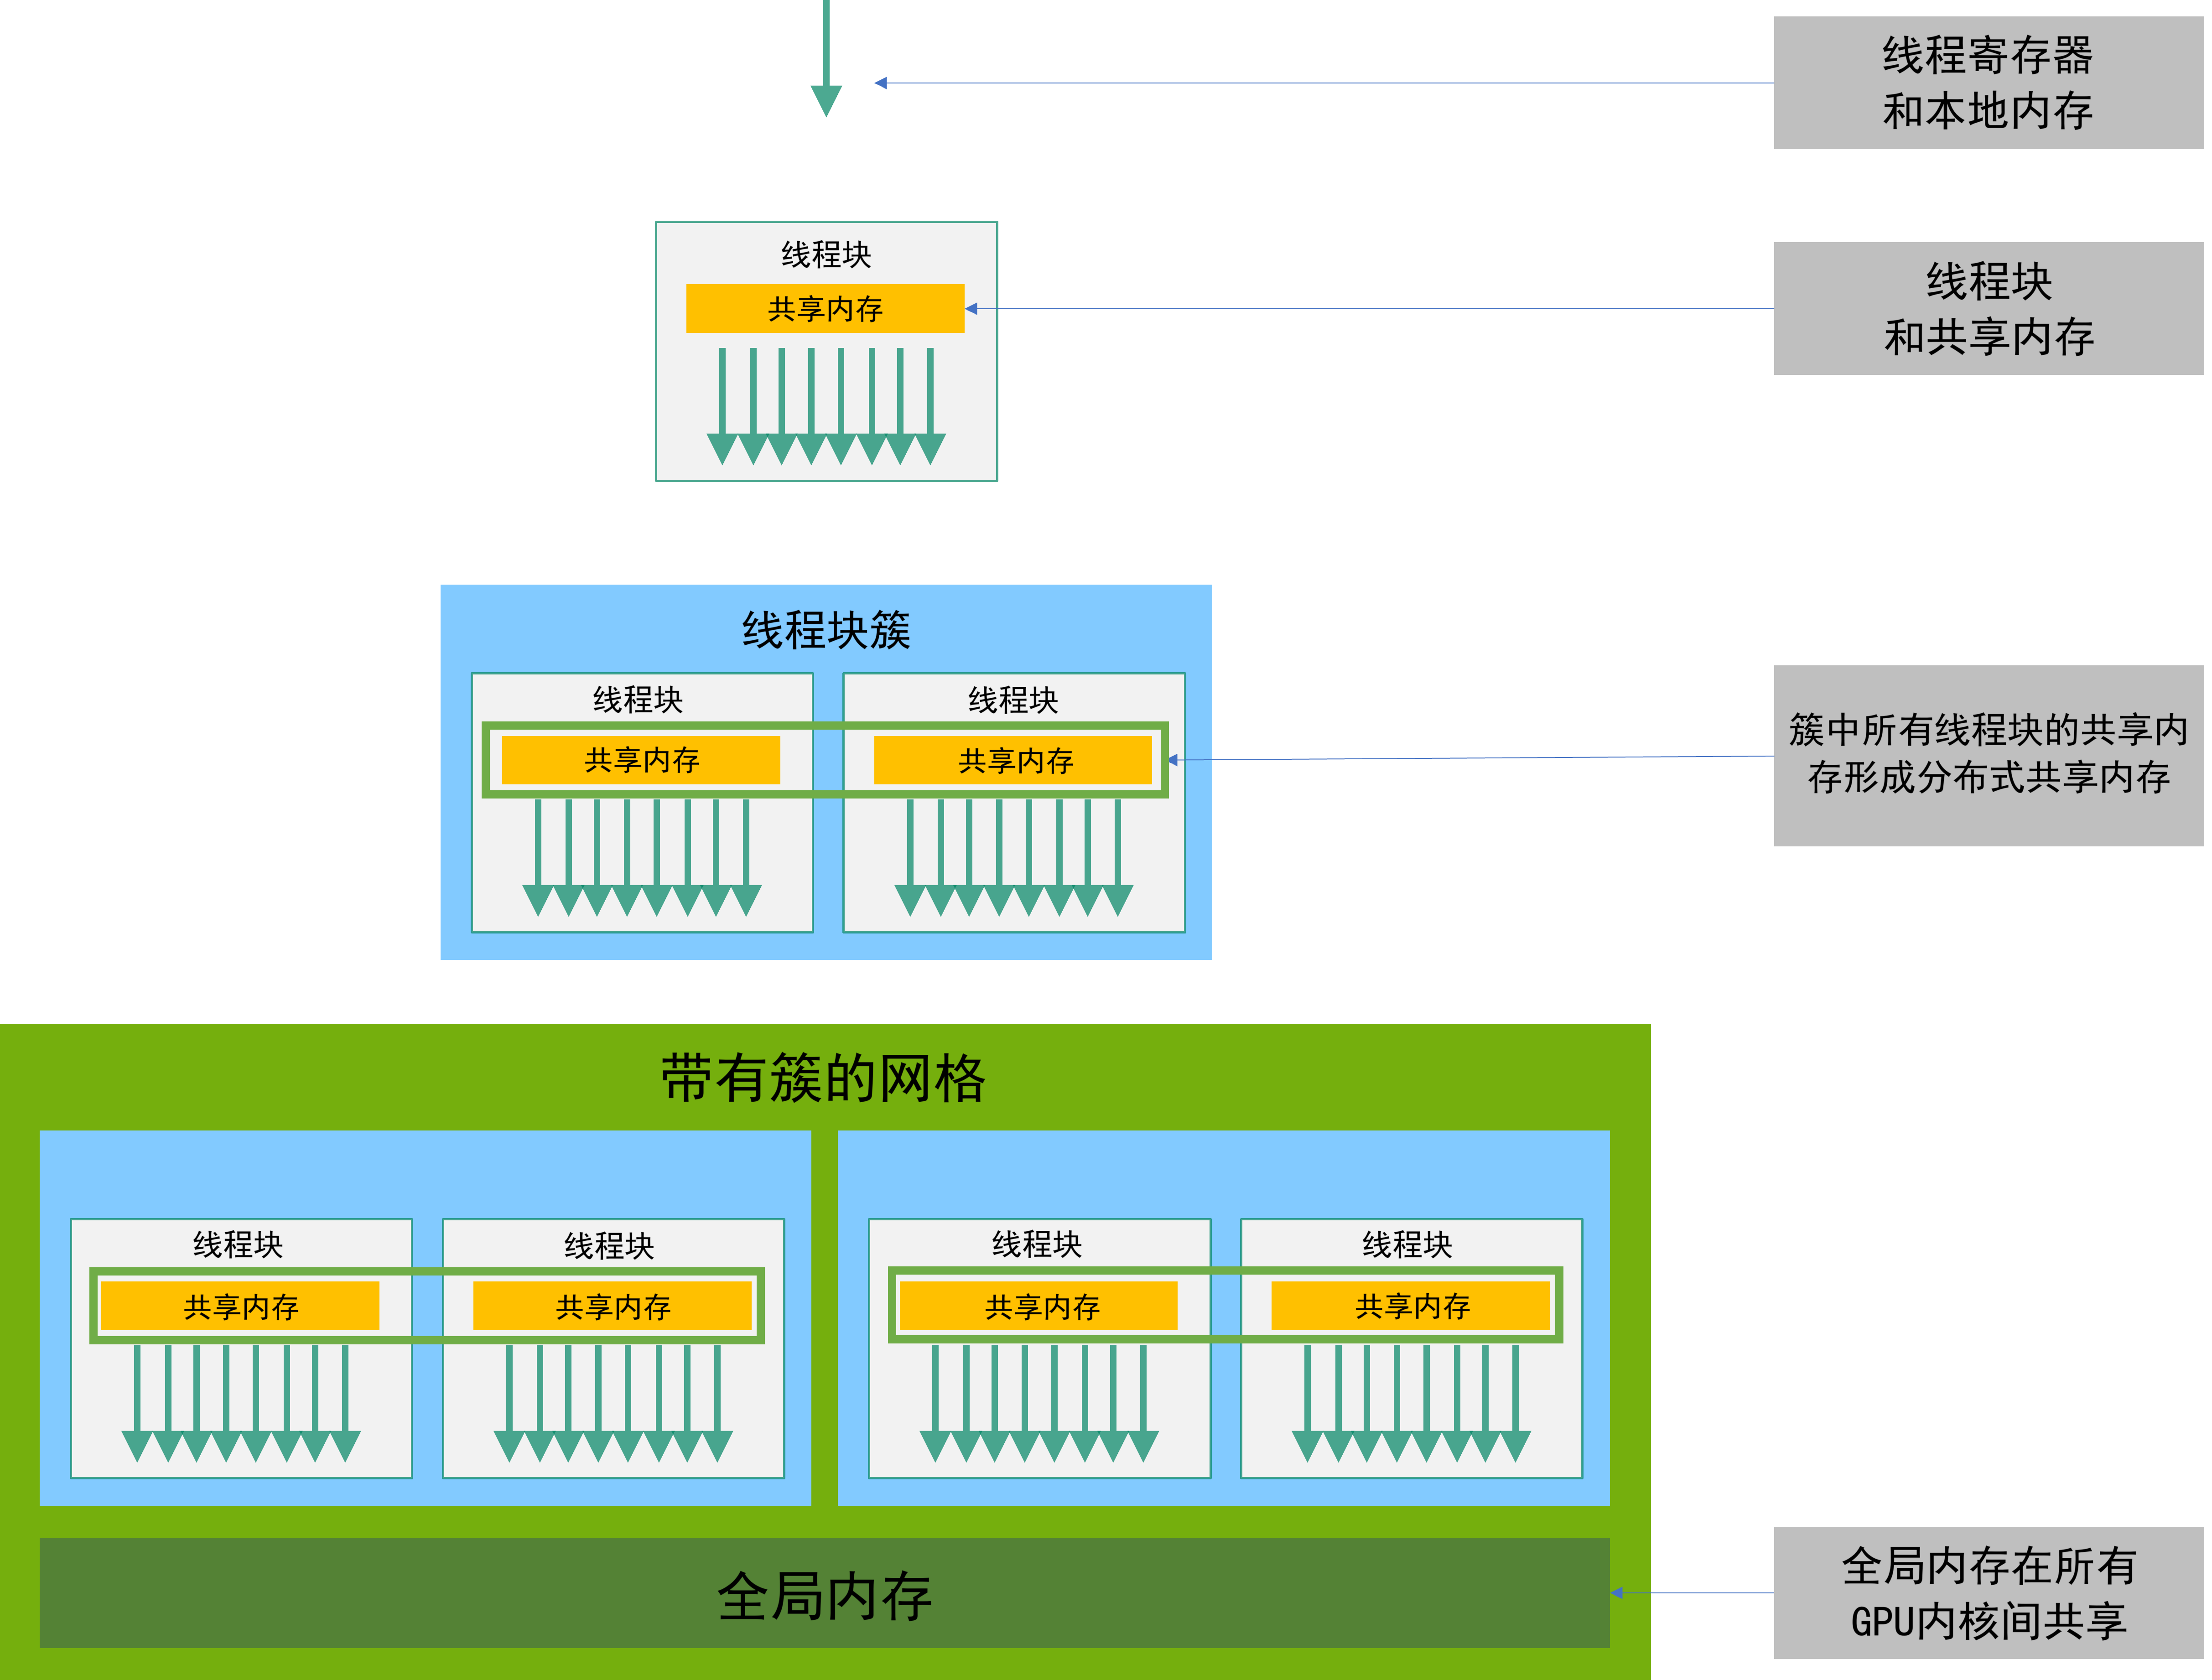
\includegraphics[width=0.9\textwidth]{figures/memory_hierarchy.png}
    \caption{GPU内存架构}
    \label{fig:memory_hierarchy}
    \note{注:GPU的分层内存模型,包括全局、共享、常量及纹理内存。}
    \end{minipage}
    % \hspace{1in}
    \begin{minipage}[t]{0.35\textwidth}
    \centering
    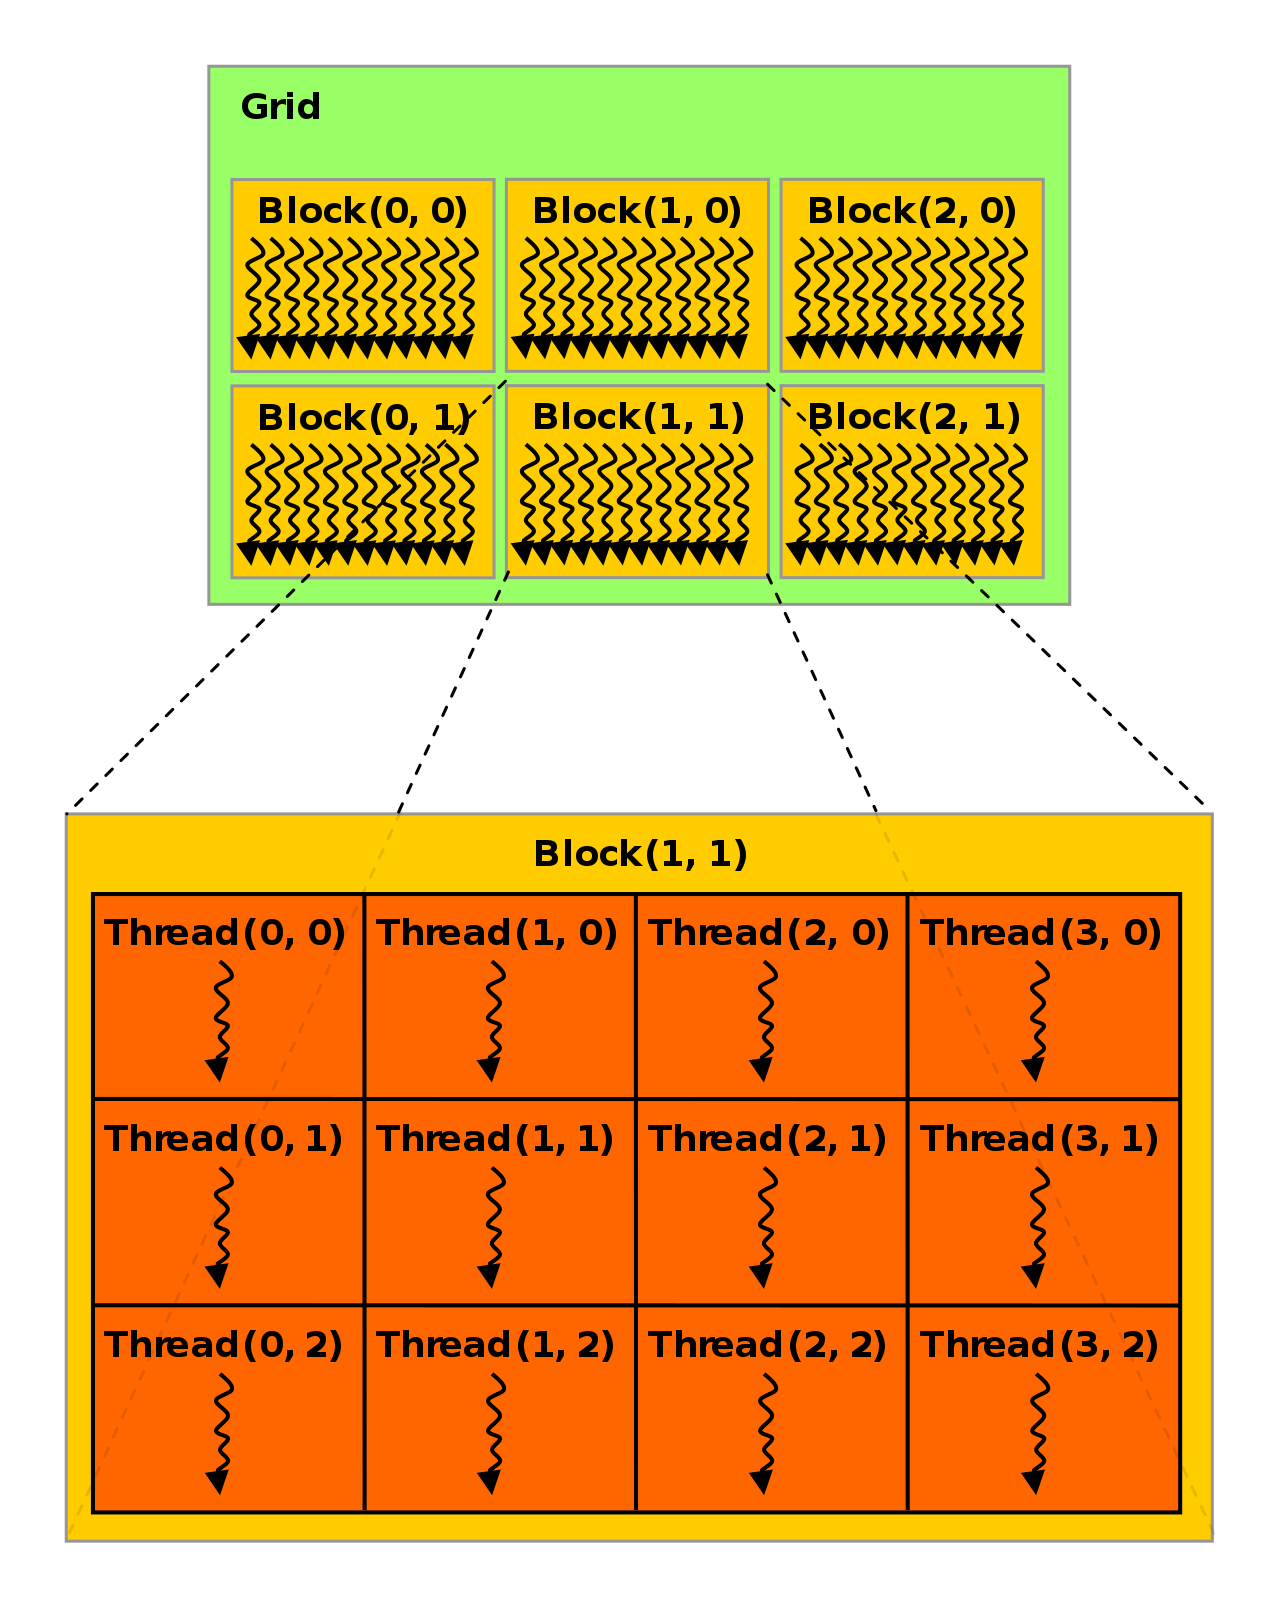
\includegraphics[width=0.9\textwidth]{figures/thread_block.png}
    \caption{GPU线程组织模型}
    \label{fig:block_thread}
    \note{注:GPU的层次化线程组织模型,包括线程、线程束、线程块和网格。}
    \end{minipage}
\end{figure}

\paragraph{GPU线程组织模型}

\par GPU采用如图\ref{fig:block_thread}\cite{nvidia_cuda}所示的层次化线程组织模型。基本单位是线程,每个
线程能够独立执行任务。在NVIDIA的架构中,32个线程组成一个线程束(Warp),这些线程同时执行
相同的指令,但是处理不同的数据。线程束进一步组织为线程块(Thread Block)。线程块内的线程
可以通过共享内存进行通信,协调它们的计算和内存访问。最后,线程块聚集在一起形成一个网格
(Grid),实现大规模的并行处理。

\subsection{CUDA编程}

\paragraph{CUDA简介}

\par CUDA(Compute Unified Device Architecture)是NVIDIA推出的并行计算平台和编程模型,
允许开发者利用NVIDIA的GPU进行通用计算。

\par CUDA提供了一系列的API,将GPU视为一个并行计算设备,允许开发者在C/C++中写并行代码,
称为内核(Kernel)。在CUDA编程模型中,程序员编写内核,指定并行线程的数量和配置,
并将内核提交给GPU执行。当线程维度为1时,线程数量和索引的计算方式如下:
\begin{equation}
    \begin{aligned}
    & \text{线程数量} = \text{blockDim.x} \times \text{gridDim.x} \\
    & \text{线程索引} = \text{blockIdx.x} \times \text{blockDim.x} + \text{threadIdx.x}
    \end{aligned}
\end{equation}

\par 此外,CUDA也支持各种高级特性,如动态并行、双精度浮点运算、原子操作和 CUDA 图等。

\paragraph{CUDA编程规范}

\par 在 CUDA 编程中,线程的组织模型与 GPU 硬件模型密切关联,这对于实时三维重建及语义分割
系统极其重要。开发过程中需要以线程束、线程块和网格的形式来管理和调度线程,以便充分利用 GPU 
的硬件特性。例如,为了避免全局内存访问的延迟,可以在共享内存中存储重建和分割过程中频繁使用的
数据,然后将其分发到各个线程\cite{nvidia_cuda}。在编程过程中,需要确保线程束内的所有线程
都执行相同的指令,以免影响系统性能。对线程束和线程块的工作方式的理解可以更有效地组织和调度线
程,避免在三维重建及语义分割过程中产生的同步和通信开销。此外,还需要考虑如何在全局内存、共享
内存和寄存器之间高效地传输和存储三维重建及语义分割所需的数据。